\chapter{Evaluation}
% take a step back and put your results from 4 into context. 
This chapter critically examines the machine learning models conceived and partially implemented in the previous chapter.
Table~\ref*{tab:evaluation_criteria} shows an overview of the evaluated criteria. These are structured according to the Goal-Question-Metric approach Mean Absolute Error (MAE) how far the predictions are from the actual output.

\captionsetup{margin={5pt,5pt}}

\begin{table}[H]
    \begin{tcolorbox}[arc=0pt,boxrule=0.5pt]
        \sisetup{group-minimum-digits = 4}
        \centering
        \caption{Overview of the goals, questions and metrics for the evaluation of artifacts following the \ac{GQM} approach.}
        \label{tab:evaluation_criteria_2}
        {\renewcommand{\arraystretch}{1}
            \begin{tabular}{p{2.5cm}p{6cm}p{3cm}}
                \toprule
                \thead{\textbf{Goal}}         & \thead{\textbf{Question}}                                                                                       & \thead{\textbf{Metric}}                              \\

                \hdashline
                \textbf{Appropriatness}       & How well does the model type fit the current task?                                                              & Prerequisites for model type                         \\

                \hdashline
                \textbf{Correctness}          & Ability of the model to perform the current task measured on the development dataset and the runtime dataset    &
                Precision, Recall, F-score                                                                                                                                                                             \\
                \hdashline
                \textbf{Relevance}            & Does the model achieve a good bias-variance tradeoff? Which means neither overfitting or unterfitting the data. & Variance of cross-validation and fit                 \\

                \hdashline
                \textbf{Robustness}           & Ability of the model to outliers, noise and other data quality issues                                           & Equalized Loss of Accuracy (ELA)                     \\

                \hdashline
                \textbf{Stability}            & Does the artifact generate repeatable results when trained on different data?                                   & Leave-one-out-cross validation stability             \\

                \hdashline
                \textbf{Interpretability}     & How well can the model be explained?                                                                            & Complexity measures (e.g., no. of parameters, depth) \\

                \hdashline
                \textbf{Resource utilization} & How much resources are required to train and run the model?                                                     & Training time, runtime, storage space                \\
                \bottomrule
            \end{tabular}
        } % renew command 
    \end{tcolorbox}
\end{table}

\section{DP1: Appropriateness}
% How well does the model type fit the current task?
% Prerequisites for model type


\section{DP2: Correctness}
% Ability of the model to perform the current task measured on the development dataset and the runtime dataset
The model must be able to perform well on the selected task.
To measure the correctness of the model, the metrics MAE, MSE and RMSE are used.
In the formulas \ref{eq:mae}, \ref{eq:mse} and \ref{eq:rmse} the variable $e_i$ is the prediction error which is the difference between the predicted value by the model the actual value.
$y_i$ is the actual value and $n$ is the number of samples in the testing data set.

The mean absolute error (MAE) and mean squared error (MSE) are the most commonly used metrics for evaluating the performance of regression models. \paragraph*{Mean Absolute Error (MAE)}

\begin{equation}
    \label{eq:mae}
    MAE = \frac{1}{n} \sum_{i=1}^{n} |e_i|
\end{equation}

The MSE is the average of the squared differences between the predicted and the actual values. The MSE is more sensitive to outliers than the MAE.

\paragraph*{Mean Squared Error (MSE)}

\begin{equation}
    \label{eq:mse}
    MSE = \frac{1}{n} \sum_{i=1}^{n} e^2
\end{equation}

The RMSE is the square root of the MSE. The RMSE is the most popular metric for evaluating the performance of regression models. The RMSE is interpretable in the same units as the response variable. The RMSE is more sensitive to outliers than the MAE.
The MAE is the average of the absolute difference between the predicted and actual values.
Additionally the $R^2$ was added to the overview. The $R^2$ is a statistical measure of how close the data are to the fitted regression line. It is also known as the coefficient of determination, or the coefficient of multiple determination for multiple regression. The value of the $R^2$ is the percentage of the response variable variation that is explained by a linear model.

\paragraph*{Root Mean Squared Error (RMSE)}

\begin{equation}
    \label{eq:rmse}
    RMSE = \sqrt{MSE}
\end{equation}

For a full overview about the performance all three metrics are sued for the evaluation.

\subsection{Goal Hierarchy}

The correctness describes the ability of the model to perform on the selected task. Concrete, the model has to predict the spring back as correct as possible. The goal hierarchy for the correctness is shown in Figure~\ref{fig:goal_hierarchie_correctness}.

\begin{figure}[H]
    \centering
    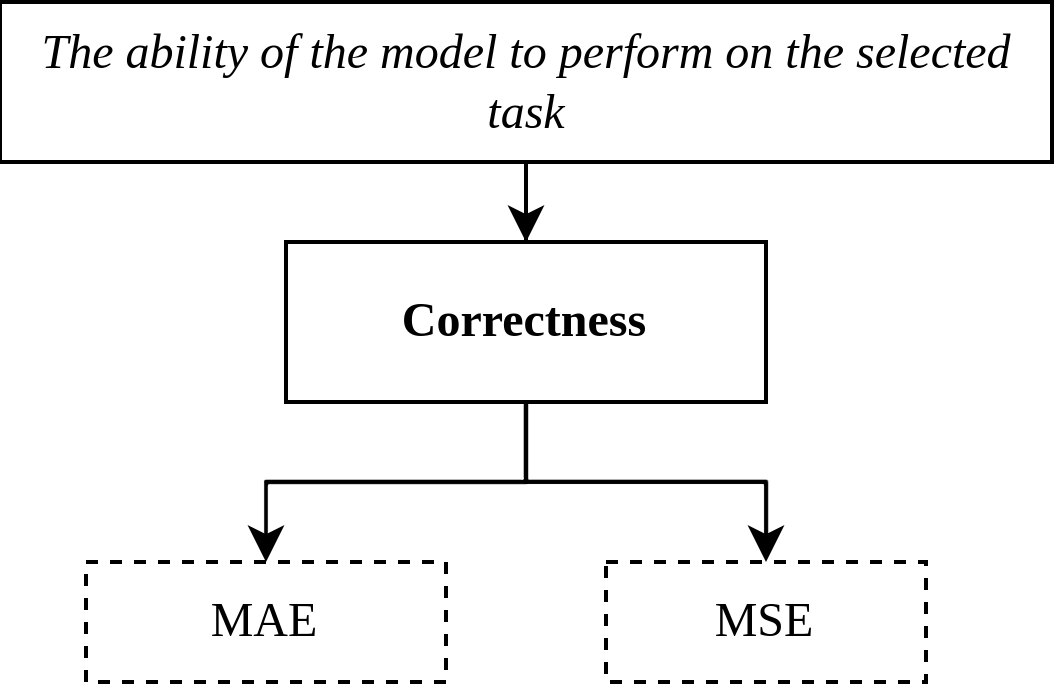
\includegraphics[width=0.6\textwidth]{goal_hierarchie_correctness}
    \caption{Goal hierarchy: Correctness}
    \label{fig:goal_hierarchie_correctness}
\end{figure}

\subsection{Results}

% Table wit hall used machine learning models and their metrics
\begin{table}[H]
    \begin{tcolorbox}[arc=0pt,boxrule=0.5pt]
        % \sisetup{group-minimum-digits = 4}
        \centering
        \begin{tabular}{llll}
            \toprule
            \thead{\textbf{Model Name}}         & \thead{\textbf{MAE}}
                                                & \thead{\textbf{MSE}}
                                                & \thead{\textbf{RMSE}}               \\
            \textbf{Random Forest (rand split)} & 0.14                  & 0.05 & 0.22 \\
            \textbf{Random Forest}              & 0.16                  & 0.04 & 0.21 \\
            \hdashline
            \textbf{Boosting}                   & 0                     & 0    & 0    \\
            \hdashline
            \textbf{Linear Regression}          & 0                     & 0    & 0    \\
            \hdashline
            \textbf{Support Vector Regression}  & 0                     & 0    & 0    \\
            \bottomrule
        \end{tabular}
        \caption{Overview of the used machine learning models and their metrics.}
        \label{tab:ml_models}
    \end{tcolorbox}
\end{table}



\section{Relevance}
% Does the model achieve a good bias-variance tradeoff? Which means neither overfitting or unterfitting the data.

% Bias variane trade-off 

The model is relevant if it is able to achieve a good bias-variance tradeoff. This means neither overfitting or unterfitting the data.
The variance of cross-validation scores gives an idea on how stable the model's performance is when it is trained an evaluated on different subsets of data.
% Chat GPT 
If the variance is low, it means that the model's performance is relatively consistent across different folds, and you can have more confidence in the evaluation. On the other hand, if the variance is high, it means that the model's performance can vary significantly depending on which data points are used as the test set, and you should be more cautious when interpreting the results.

If the variance is low, it means that the model's performance is relatively consistent across different folds, and you can have more confidence in the evaluation. On the other hand, if the variance is high, it means that the model's performance can vary significantly depending on which data points are used as the test set, and you should be more cautious when interpreting the results.

\paragraph*{Variance of cross-validation and fit}

\begin{equation}
    \label{eq:variance_cross}
    Variance_{cross} = \frac{1}{n} \sum_{i=1}^{n} (\hat{y}_i - y_i)^2
\end{equation}

\paragraph*{R2}

\begin{equation}
    \label{eq:r2}
    R^2 = 1 - \frac{Variance_{cross}}{Variance_{fit}}
\end{equation}

Table~\ref*{tab:ml_models_relevance} shows the variance of cross-validation and the $R^2$ for all used machine learning models.
To calculate the variance of cross-validation  the variance of Scikit-Learn's \texttt{cross\_val\_score} was calculated. five-fold cross-validation was used to calculate the variance of cross-validation. The $R^2$ was calculated with the formula~\ref{eq:r2}.

\begin{table}[H]
    \begin{tcolorbox}[arc=0pt,boxrule=0.5pt]
        % \sisetup{group-minimum-digits = 4}
        \centering
        \begin{tabular}{lll}
            \toprule
            \thead{\textbf{Model Name}} & \thead{\textbf{Variance of CV}}
                                        & \thead{\textbf{$R^2$}}                  \\
            \toprule
            \textbf{Random Forest}      & 0.034                           & 0.771 \\
            \hdashline
            \textbf{Boosting}           & 0.000                           & 0.000 \\
            \hdashline
            \textbf{Linear Regression}  & 0.000                           & 0.000 \\
            \hdashline
            \textbf{Support Vector}     & 0.000                           & 0.000 \\
            \bottomrule
        \end{tabular}
        \caption{Overview of the used machine learning models and their metrics.}
        \label{tab:ml_models_relevance}
    \end{tcolorbox}
\end{table}

% Variance of cross-validation and fit
% -> Fit -> R2


\section{Robustness}
% Ability of the model to outliers, noise and other data quality issues
% Variance of cross-validation, fit

% Equalized Loss of Accuracy (ELA) 

Robustness is the ability of the model to handle outliers, noise and other data quality issues. \cite[p. 16]{saez_evaluatingclassifierbehavior_2016}
To classification problems there is already an established metric to measure the robustness of the model. This metric is the Equalized Loss of Accuracy (ELA). \cite[p. 1]{saez_evaluatingclassifierbehavior_2016}
There is no direct equivalent of the ELA measure for regression tasks, since the ELA measure is specific to classification. However, there are a number of ways to evaluate the performance of regression models, including mean squared error (MSE), mean absolute error (MAE), and root mean squared error (RMSE). You can use these measures to compare the performance of different regression models on a given task.
Also the $R^2$ can be used to measure the robustness of the model.

\subsubsection*{Notes}

\begin{itemize}
    \item An alternative metric instead of ELA could be the approach of Scher and Trügler. But it would be necessary to implement the metric in Python.
\end{itemize}


\section{Stability}
% Does the artifact generate repeatable results when trained on different data?
% Leave-one-out cross-validation stability 
Stability is the ability of the model to generate repeatable results when trained on different data. \cite[p. 16]{siebert_constructionqualitymodel_}
To measure the stability of the model, leave-one-out cross-validation (\ac{LOOCV}) was used.
\ac{LOOCV} is


\paragraph*{Leave-one-out cross-validation \ac{LOOCV}}

\begin{equation}
    \label{eq:loo}
    LOO = \frac{1}{n} \sum_{i=1}^{n} \frac{1}{\hat{y}_i} |y_i - \hat{y}_i|
\end{equation}

\ac{LOOCV} is another method that is commonly used. It can be thought of as a type of k-fold cross-validation where each fold consists of a single sample. During each split, a single data point is selected to be the test set. This method can be very time-consuming, especially for large datasets, but it may provide more accurate estimates for small datasets. \cite[p. 257-258]{muller_introductionmachinelearning_2016}

The variance of all \ac{CV} scores is calculated with the formula~\ref{eq:variance_cross}.
A low variance indicates that the model is stable which means that the model's performance is consistent across different training and testing sets. This is generally  a desirable property for a model to have, as it suggest that the model ist not overfitting to the training data and is able to generalize well to unseen data.

On the other hand, a high variances indicates an unstable model and is a sign of overfitting, as the model may be to closely tied to the training data and not generalize well to unseen data.

\subsection{Results}

\begin{table}[H]
    \begin{tcolorbox}[arc=0pt,boxrule=0.5pt]
        % \sisetup{group-minimum-digits = 4}
        \centering
        \begin{tabular}{ll}
            \toprule
            \thead{\textbf{Model Name}} & \thead{\textbf{Variance of \ac{LOOCV}}}
            \\
            \toprule
            \textbf{\ac{RF}}            & 0.053                                   \\
            \hdashline
            \textbf{RFB}                & 0.000                                   \\
            \hdashline
            \textbf{LR}                 & 0.000                                   \\
            \hdashline
            \textbf{\ac{SVM}}           & 0.000                                   \\
            \bottomrule
        \end{tabular}
        \caption{Overview of the used machine learning models and their metrics.}
        \label{tab:ml_models_statbility}
    \end{tcolorbox}
\end{table}

\textit{Explanation of the results}

\subsubsection*{\textit{Notes}}

\begin{itemize}
    \item \textit{Why exactly does the variance of LOOCV measure the robustness and the variance of CV the relevane?}
\end{itemize}

\section{Interpretability}
% How well can the model be explained?
% Complexity measures (e.g., no. of parameters, depth)
% R^2 value ???? 
Interpretability refers to the ease with which humans can understand and make sense of the decisions made by a trained machine learning model. \cite[p. 16]{siebert_constructionqualitymodel_} It is the extent to which the inner workings of the model and the reasoning behind its predictions can be understood by human users. Good interpretability is important because it allows users to trust and rely on the model, and it can also help with debugging and improving the model.
To measure the interpretability of the model, the following metrics are used:

\paragraph*{The number of parameters in the model}
Measured as integer, representing the total number of parameters in the model.
Models with more parameters are generally more complex and more prone to overfitting

\paragraph*{Depth of the model}
Measured as an integer, representing the number of layers in the model.
A model with many layers, is generally more complex than a shallow network with fewer layers.

\paragraph*{Inference time}
Measured in milliseconds. Time it takes to make a prediction.
A model that takes longer to make predictions may be more complex than a model that is able to make predictions more quickly.

\paragraph*{Level of interpretability}
\textit{Harder to measure but some ideas: }
\begin{itemize}
    \item \textit{Partial dependence plots: These plots show the relationship between a single feature and the model's predictions, holding all other features constant. This can help to identify which features are most important for the model and how they influence the predictions.}
    \item \textit{LIME (Local Interpretable Model-Agnostic Explanations): This is a method for explaining the predictions of any black-box classifier. It works by training an interpretable model locally around the prediction of interest, and using this local model to explain the prediction of the black-box model.}
    \item \textit{SHAP (SHapley Additive exPlanations): This is another method for explaining the predictions of black-box models. It works by assigning importance to each feature based on its contribution to the model's prediction.}

\end{itemize}


\paragraph*{Amount of training data required}
\textit{Will be the same for all models so this metric may not be used.}

\subsection{Results}

\begin{table}[H]
    \begin{tcolorbox}[arc=0pt,boxrule=0.5pt]
        % \sisetup{group-minimum-digits = 4}
        \centering
        \begin{tabular}{lllll}
            \toprule
            \thead{\textbf{Model Name}} & \thead{\textbf{Number Parameters}}
                                        & \thead{\textbf{Depth}}             & \thead{\textbf{Inference}}
                                        & \thead{\textbf{Interpretability}}
            \\
            \toprule
            \textbf{\ac{RF}}            & 0.000                              & 0.000                      & 0.000 & 0.000 \\
            \hdashline
            \textbf{\ac{RFB}}           & 0.000                              & 0.000                      & 0.000 & 0.000 \\
            \hdashline
            \textbf{LR}                 & 0.000                              & 0.000                      & 0.000 & 0.000 \\
            \hdashline
            \textbf{SVM}                & 0.000                              & 0.000                      & 0.000 & 0.000 \\
            \bottomrule
        \end{tabular}
        \caption{Overview of the used machine learning models and their metrics.}
        \label{tab:ml_models_statbility}
    \end{tcolorbox}
\end{table}

\textit{Explanation of the results}


\section{Resource utilization}
% How much resources are required to train and run the model?
% Training time, runtime, storage space

To measure the resource utilization of the model, the following metrics are used:

% From Copilot
\paragraph*{Training time}
Measured in seconds. Refers to the time it takes to train the model.
Training a model requires resources such as memory, CPU, and GPU, therefore the longer it takes to train a model, the more resources are required. According to resources utilization a shorter training time is desirable.

The training time is measured using the \texttt{time.time} function in python. The function returns the time in seconds since the epoch. The time is measured before and after the model is fitted. The difference between the two times is the training time.

\paragraph*{Runtime}
Measured in milliseconds. It refers to the time it takes to make a prediction on data once it has been trained.
It is an important measure not only for real-world application but also a faster runtime uses less resources and is therefore more efficient.

The runtime is measured using the \texttt{time.time}  function in python.  On value is picked out of the test set and the time is measured before and after the prediction is made. The difference between the two times is the runtime.

\paragraph*{Storage space}
Measured in kilobytes. It refers to the amount of storage space required to store the model.
The more storage space required to store the model, the more resources are required to store it. Therefore, a smaller storage space is desirable.

\begin{table}[H]
    \begin{tcolorbox}[arc=0pt,boxrule=0.5pt]
        % \sisetup{group-minimum-digits = 4}
        \centering
        \begin{tabular}{llll}
            \toprule
            \thead{\textbf{Model Name}} & {\thead{\textbf{Training time}\\ \unit[]{s}}}
                                        & {\thead{\textbf{Runtime}\\ \unit[]{ms}}}       & {\thead{\textbf{Storage space}\\ \unit{kb}}}
            \\
            \toprule
            \textbf{\ac{RF}}            & 0.0222 & 2.0275 & 80.2                                                                   \\
            \hdashline
            \textbf{LR}                 & 0.000                          & 0.000                          & 0.000 \\
            \hdashline
            \textbf{SVM}                & 0.000                          & 0.000                          & 0.000 \\
            \bottomrule
        \end{tabular}
        \caption{Overview of the used machine learning models and their metrics.}
        \label{tab:ml_models_statbility}
    \end{tcolorbox}
\end{table}


\section{Summary}
Using the evaluation metrics described in the previous sections, the following results were achieved.
